\documentclass[14pt]{extbook}
\usepackage{multicol, enumerate, enumitem, hyperref, color, soul, setspace, parskip, fancyhdr} %General Packages
\usepackage{amssymb, amsthm, amsmath, latexsym, units, mathtools} %Math Packages
\everymath{\displaystyle} %All math in Display Style
% Packages with additional options
\usepackage[headsep=0.5cm,headheight=12pt, left=1 in,right= 1 in,top= 1 in,bottom= 1 in]{geometry}
\usepackage[usenames,dvipsnames]{xcolor}
\usepackage{dashrule}  % Package to use the command below to create lines between items
\newcommand{\litem}[1]{\item#1\hspace*{-1cm}\rule{\textwidth}{0.4pt}}
\pagestyle{fancy}
\lhead{Progress Quiz 4}
\chead{}
\rhead{Version ALL}
\lfoot{5346-5907}
\cfoot{}
\rfoot{Summer C 2021}
\begin{document}

\begin{enumerate}
\litem{
Factor the quadratic below. Then, choose the intervals that contain the constants in the form $(ax+b)(cx+d); b \leq d.$\[ 54x^{2} +75 x + 25 \]\begin{enumerate}[label=\Alph*.]
\item \( a \in [17.97, 18.27], \hspace*{5mm} b \in [1, 10], \hspace*{5mm} c \in [2.94, 3.17], \text{ and } \hspace*{5mm} d \in [3, 9] \)
\item \( a \in [2.63, 3.64], \hspace*{5mm} b \in [1, 10], \hspace*{5mm} c \in [17.76, 18.39], \text{ and } \hspace*{5mm} d \in [3, 9] \)
\item \( a \in [7.53, 9.28], \hspace*{5mm} b \in [1, 10], \hspace*{5mm} c \in [5.06, 6.19], \text{ and } \hspace*{5mm} d \in [3, 9] \)
\item \( a \in [0.01, 2.03], \hspace*{5mm} b \in [25, 32], \hspace*{5mm} c \in [0.85, 1.82], \text{ and } \hspace*{5mm} d \in [44, 46] \)
\item \( \text{None of the above.} \)

\end{enumerate} }
\litem{
Write the equation of the graph presented below in the form $f(x)=ax^2+bx+c$, assuming  $a=1$ or $a=-1$. Then, choose the intervals that $a, b,$ and $c$ belong to.
\begin{center}
    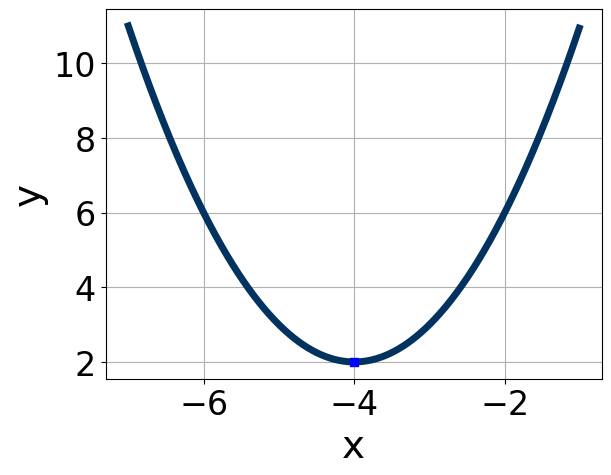
\includegraphics[width=0.5\textwidth]{../Figures/quadraticGraphToEquationA.png}
\end{center}
\begin{enumerate}[label=\Alph*.]
\item \( a \in [1, 3], \hspace*{5mm} b \in [-8, -6], \text{ and } \hspace*{5mm} c \in [17, 19] \)
\item \( a \in [1, 3], \hspace*{5mm} b \in [-8, -6], \text{ and } \hspace*{5mm} c \in [12, 15] \)
\item \( a \in [-2, 0], \hspace*{5mm} b \in [7, 12], \text{ and } \hspace*{5mm} c \in [-15, -13] \)
\item \( a \in [1, 3], \hspace*{5mm} b \in [7, 12], \text{ and } \hspace*{5mm} c \in [17, 19] \)
\item \( a \in [-2, 0], \hspace*{5mm} b \in [-8, -6], \text{ and } \hspace*{5mm} c \in [-15, -13] \)

\end{enumerate} }
\litem{
Factor the quadratic below. Then, choose the intervals that contain the constants in the form $(ax+b)(cx+d); b \leq d.$\[ 24x^{2} +38 x + 15 \]\begin{enumerate}[label=\Alph*.]
\item \( a \in [3.6, 4.3], \hspace*{5mm} b \in [2, 5], \hspace*{5mm} c \in [3.7, 8.4], \text{ and } \hspace*{5mm} d \in [2, 8] \)
\item \( a \in [-2.2, 2.5], \hspace*{5mm} b \in [16, 22], \hspace*{5mm} c \in [0.2, 2.1], \text{ and } \hspace*{5mm} d \in [18, 23] \)
\item \( a \in [4.3, 9.5], \hspace*{5mm} b \in [2, 5], \hspace*{5mm} c \in [2.5, 3.1], \text{ and } \hspace*{5mm} d \in [2, 8] \)
\item \( a \in [-2.2, 2.5], \hspace*{5mm} b \in [2, 5], \hspace*{5mm} c \in [17.7, 21.1], \text{ and } \hspace*{5mm} d \in [2, 8] \)
\item \( \text{None of the above.} \)

\end{enumerate} }
\litem{
Write the equation of the graph presented below in the form $f(x)=ax^2+bx+c$, assuming  $a=1$ or $a=-1$. Then, choose the intervals that $a, b,$ and $c$ belong to.
\begin{center}
    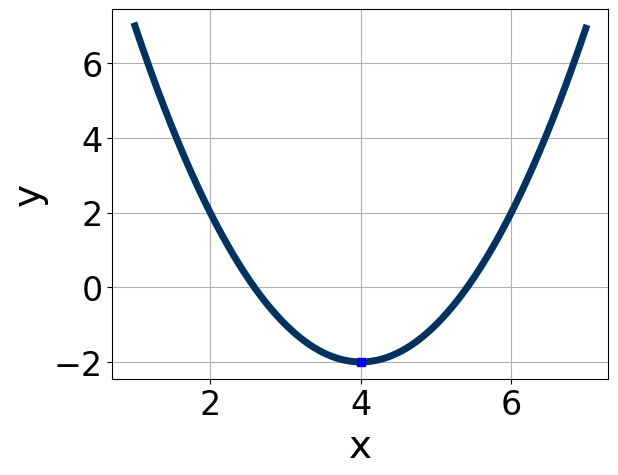
\includegraphics[width=0.5\textwidth]{../Figures/quadraticGraphToEquationCopyA.png}
\end{center}
\begin{enumerate}[label=\Alph*.]
\item \( a \in [0, 3], \hspace*{5mm} b \in [-11, -7], \text{ and } \hspace*{5mm} c \in [12, 16] \)
\item \( a \in [0, 3], \hspace*{5mm} b \in [7, 10], \text{ and } \hspace*{5mm} c \in [12, 16] \)
\item \( a \in [-1, 0], \hspace*{5mm} b \in [7, 10], \text{ and } \hspace*{5mm} c \in [-18, -17] \)
\item \( a \in [0, 3], \hspace*{5mm} b \in [7, 10], \text{ and } \hspace*{5mm} c \in [17, 20] \)
\item \( a \in [-1, 0], \hspace*{5mm} b \in [-11, -7], \text{ and } \hspace*{5mm} c \in [-18, -17] \)

\end{enumerate} }
\litem{
Solve the quadratic equation below. Then, choose the intervals that the solutions belong to, with $x_1 \leq x_2$ (if they exist).\[ -19x^{2} -10 x + 3 = 0 \]\begin{enumerate}[label=\Alph*.]
\item \( x_1 \in [-0.47, 1] \text{ and } x_2 \in [0.36, 0.79] \)
\item \( x_1 \in [-18.58, -17.34] \text{ and } x_2 \in [17.55, 18.46] \)
\item \( x_1 \in [-5.15, -3.78] \text{ and } x_2 \in [13.22, 15.05] \)
\item \( x_1 \in [-1.53, -0.48] \text{ and } x_2 \in [-0.67, 0.65] \)
\item \( \text{There are no Real solutions.} \)

\end{enumerate} }
\litem{
Graph the equation below.\[ f(x) = (x+2)^2 + 10 \]\begin{enumerate}[label=\Alph*.]
\begin{multicols}{2}\item 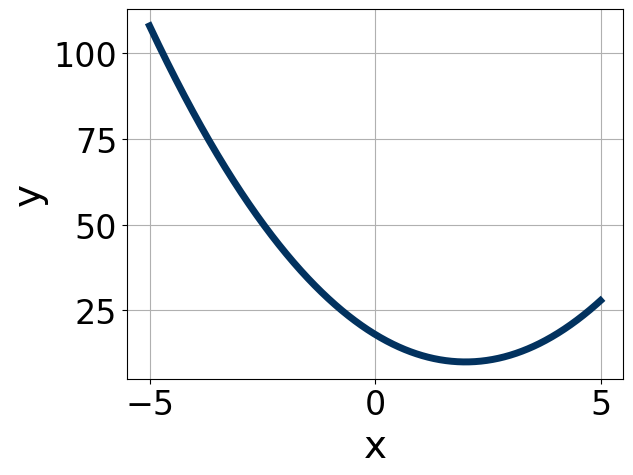
\includegraphics[width = 0.3\textwidth]{../Figures/quadraticEquationToGraphCopyAA.png}\item 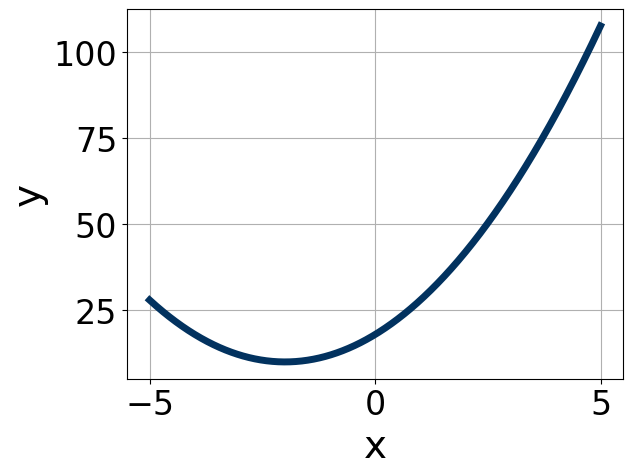
\includegraphics[width = 0.3\textwidth]{../Figures/quadraticEquationToGraphCopyBA.png}\item 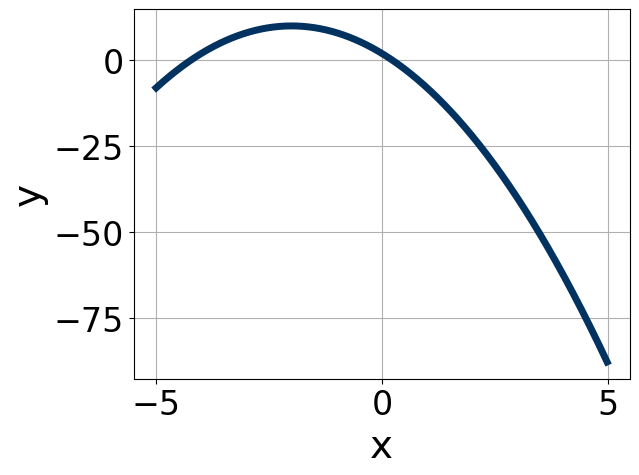
\includegraphics[width = 0.3\textwidth]{../Figures/quadraticEquationToGraphCopyCA.png}\item 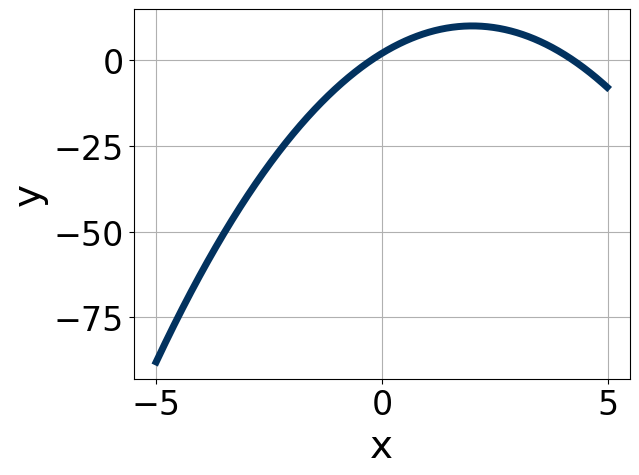
\includegraphics[width = 0.3\textwidth]{../Figures/quadraticEquationToGraphCopyDA.png}\end{multicols}\item None of the above.
\end{enumerate} }
\litem{
Solve the quadratic equation below. Then, choose the intervals that the solutions belong to, with $x_1 \leq x_2$ (if they exist).\[ -15x^{2} -13 x + 4 = 0 \]\begin{enumerate}[label=\Alph*.]
\item \( x_1 \in [-0.3, 0.4] \text{ and } x_2 \in [0.4, 2.8] \)
\item \( x_1 \in [-1.4, -0.91] \text{ and } x_2 \in [0, 1] \)
\item \( x_1 \in [-21.08, -19.8] \text{ and } x_2 \in [19.5, 20.1] \)
\item \( x_1 \in [-3.72, -3.56] \text{ and } x_2 \in [15.5, 17.7] \)
\item \( \text{There are no Real solutions.} \)

\end{enumerate} }
\litem{
Solve the quadratic equation below. Then, choose the intervals that the solutions $x_1$ and $x_2$ belong to, with $x_1 \leq x_2$.\[ 15x^{2} -2 x -24 = 0 \]\begin{enumerate}[label=\Alph*.]
\item \( x_1 \in [-1.34, -0.52] \text{ and } x_2 \in [1.19, 1.54] \)
\item \( x_1 \in [-18.42, -16.06] \text{ and } x_2 \in [19.15, 22.14] \)
\item \( x_1 \in [-0.61, 0.88] \text{ and } x_2 \in [3.23, 4.34] \)
\item \( x_1 \in [-3.25, -1.8] \text{ and } x_2 \in [0.52, 0.91] \)
\item \( x_1 \in [-7.68, -4.82] \text{ and } x_2 \in [-0.11, 0.28] \)

\end{enumerate} }
\litem{
Solve the quadratic equation below. Then, choose the intervals that the solutions $x_1$ and $x_2$ belong to, with $x_1 \leq x_2$.\[ 20x^{2} +21 x -54 = 0 \]\begin{enumerate}[label=\Alph*.]
\item \( x_1 \in [-2.36, -1.61] \text{ and } x_2 \in [0.71, 1.78] \)
\item \( x_1 \in [-45.17, -43.41] \text{ and } x_2 \in [23.82, 24.07] \)
\item \( x_1 \in [-1.74, -0.72] \text{ and } x_2 \in [2.86, 3.92] \)
\item \( x_1 \in [-6.09, -3.29] \text{ and } x_2 \in [0.49, 1.1] \)
\item \( x_1 \in [-9.23, -8.95] \text{ and } x_2 \in [-0.1, 0.31] \)

\end{enumerate} }
\litem{
Graph the equation below.\[ f(x) = -(x-3)^2 - 13 \]\begin{enumerate}[label=\Alph*.]
\begin{multicols}{2}\item 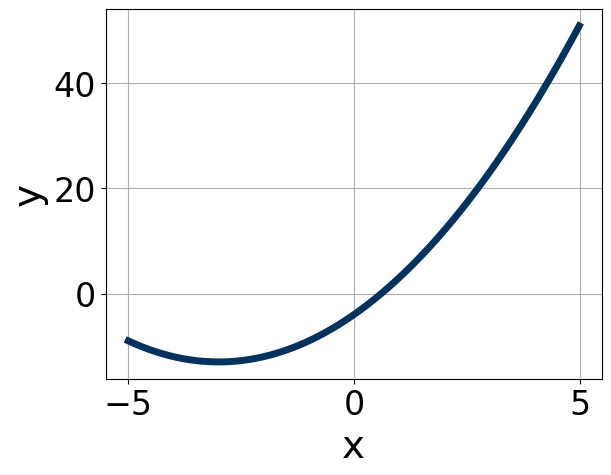
\includegraphics[width = 0.3\textwidth]{../Figures/quadraticEquationToGraphAA.png}\item 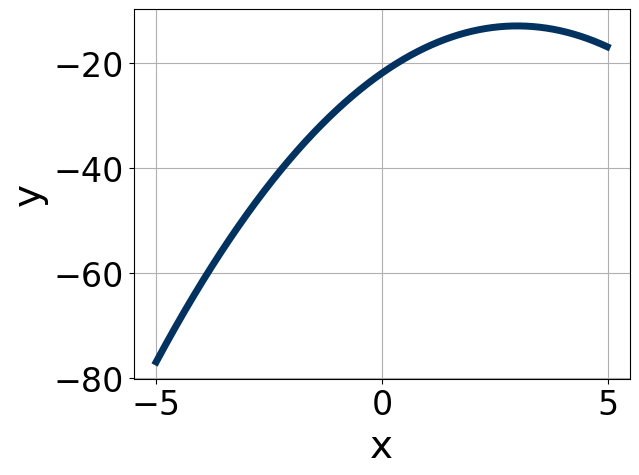
\includegraphics[width = 0.3\textwidth]{../Figures/quadraticEquationToGraphBA.png}\item 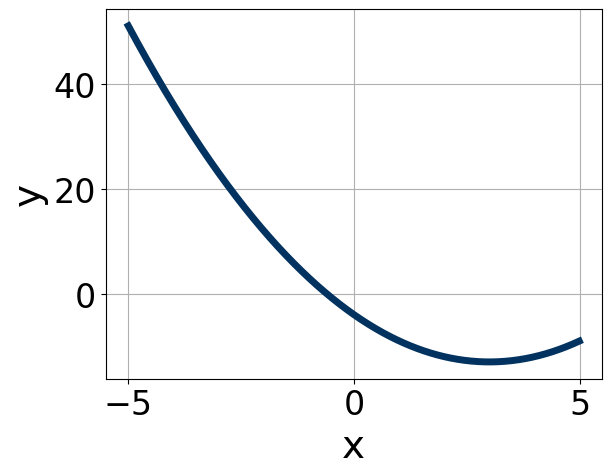
\includegraphics[width = 0.3\textwidth]{../Figures/quadraticEquationToGraphCA.png}\item 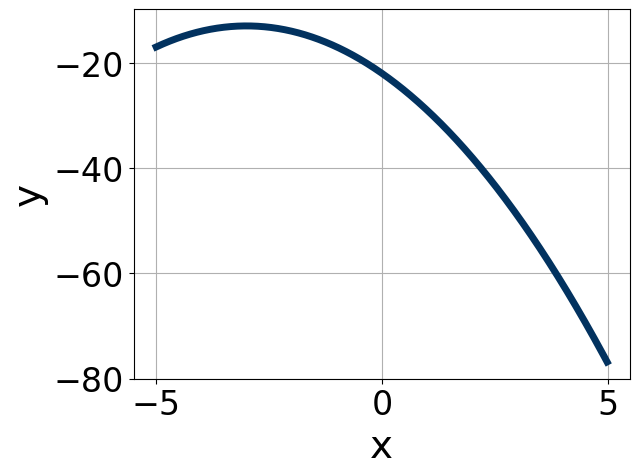
\includegraphics[width = 0.3\textwidth]{../Figures/quadraticEquationToGraphDA.png}\end{multicols}\item None of the above.
\end{enumerate} }
\litem{
Factor the quadratic below. Then, choose the intervals that contain the constants in the form $(ax+b)(cx+d); b \leq d.$\[ 36x^{2} -60 x + 25 \]\begin{enumerate}[label=\Alph*.]
\item \( a \in [-0.9, 1.5], \hspace*{5mm} b \in [-37, -29], \hspace*{5mm} c \in [0.51, 1.23], \text{ and } \hspace*{5mm} d \in [-36, -26] \)
\item \( a \in [16.5, 22.4], \hspace*{5mm} b \in [-9, -3], \hspace*{5mm} c \in [1.24, 2.9], \text{ and } \hspace*{5mm} d \in [-6, 0] \)
\item \( a \in [1.1, 5], \hspace*{5mm} b \in [-9, -3], \hspace*{5mm} c \in [10.55, 12.05], \text{ and } \hspace*{5mm} d \in [-6, 0] \)
\item \( a \in [4.2, 11.2], \hspace*{5mm} b \in [-9, -3], \hspace*{5mm} c \in [5.15, 6.42], \text{ and } \hspace*{5mm} d \in [-6, 0] \)
\item \( \text{None of the above.} \)

\end{enumerate} }
\litem{
Write the equation of the graph presented below in the form $f(x)=ax^2+bx+c$, assuming  $a=1$ or $a=-1$. Then, choose the intervals that $a, b,$ and $c$ belong to.
\begin{center}
    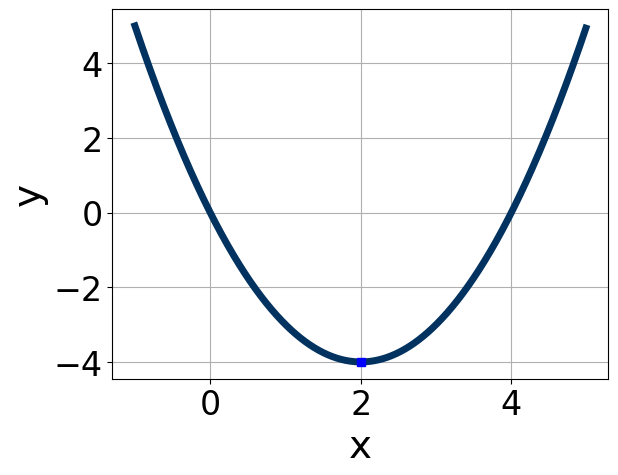
\includegraphics[width=0.5\textwidth]{../Figures/quadraticGraphToEquationB.png}
\end{center}
\begin{enumerate}[label=\Alph*.]
\item \( a \in [-2, 0], \hspace*{5mm} b \in [4, 5], \text{ and } \hspace*{5mm} c \in [-9, -5] \)
\item \( a \in [1, 5], \hspace*{5mm} b \in [4, 5], \text{ and } \hspace*{5mm} c \in [-1, 6] \)
\item \( a \in [-2, 0], \hspace*{5mm} b \in [-5, -3], \text{ and } \hspace*{5mm} c \in [-9, -5] \)
\item \( a \in [1, 5], \hspace*{5mm} b \in [-5, -3], \text{ and } \hspace*{5mm} c \in [-1, 6] \)
\item \( a \in [1, 5], \hspace*{5mm} b \in [4, 5], \text{ and } \hspace*{5mm} c \in [6, 9] \)

\end{enumerate} }
\litem{
Factor the quadratic below. Then, choose the intervals that contain the constants in the form $(ax+b)(cx+d); b \leq d.$\[ 81x^{2} -81 x + 20 \]\begin{enumerate}[label=\Alph*.]
\item \( a \in [8.8, 12.9], \hspace*{5mm} b \in [-8, -1], \hspace*{5mm} c \in [7.6, 10.7], \text{ and } \hspace*{5mm} d \in [-5, -1] \)
\item \( a \in [0.7, 2.9], \hspace*{5mm} b \in [-48, -41], \hspace*{5mm} c \in [-2.4, 1.9], \text{ and } \hspace*{5mm} d \in [-40, -32] \)
\item \( a \in [26, 30.4], \hspace*{5mm} b \in [-8, -1], \hspace*{5mm} c \in [2, 4.6], \text{ and } \hspace*{5mm} d \in [-5, -1] \)
\item \( a \in [1.4, 3.8], \hspace*{5mm} b \in [-8, -1], \hspace*{5mm} c \in [25.5, 27.8], \text{ and } \hspace*{5mm} d \in [-5, -1] \)
\item \( \text{None of the above.} \)

\end{enumerate} }
\litem{
Write the equation of the graph presented below in the form $f(x)=ax^2+bx+c$, assuming  $a=1$ or $a=-1$. Then, choose the intervals that $a, b,$ and $c$ belong to.
\begin{center}
    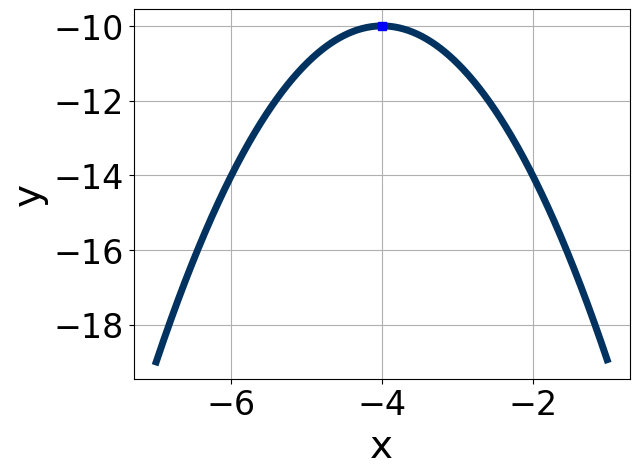
\includegraphics[width=0.5\textwidth]{../Figures/quadraticGraphToEquationCopyB.png}
\end{center}
\begin{enumerate}[label=\Alph*.]
\item \( a \in [-2, 0], \hspace*{5mm} b \in [-8, -7], \text{ and } \hspace*{5mm} c \in [-27, -23] \)
\item \( a \in [-2, 0], \hspace*{5mm} b \in [8, 11], \text{ and } \hspace*{5mm} c \in [-6, -4] \)
\item \( a \in [1, 4], \hspace*{5mm} b \in [-8, -7], \text{ and } \hspace*{5mm} c \in [6, 7] \)
\item \( a \in [1, 4], \hspace*{5mm} b \in [8, 11], \text{ and } \hspace*{5mm} c \in [6, 7] \)
\item \( a \in [-2, 0], \hspace*{5mm} b \in [8, 11], \text{ and } \hspace*{5mm} c \in [-27, -23] \)

\end{enumerate} }
\litem{
Solve the quadratic equation below. Then, choose the intervals that the solutions belong to, with $x_1 \leq x_2$ (if they exist).\[ -15x^{2} -12 x + 8 = 0 \]\begin{enumerate}[label=\Alph*.]
\item \( x_1 \in [-7.8, -4.5] \text{ and } x_2 \in [17.7, 19.6] \)
\item \( x_1 \in [-26.2, -24.5] \text{ and } x_2 \in [23.4, 24.7] \)
\item \( x_1 \in [-2.3, -0.5] \text{ and } x_2 \in [0.3, 1] \)
\item \( x_1 \in [-0.9, 0.4] \text{ and } x_2 \in [0.6, 1.4] \)
\item \( \text{There are no Real solutions.} \)

\end{enumerate} }
\litem{
Graph the equation below.\[ f(x) = -(x-4)^2 + 16 \]\begin{enumerate}[label=\Alph*.]
\begin{multicols}{2}\item 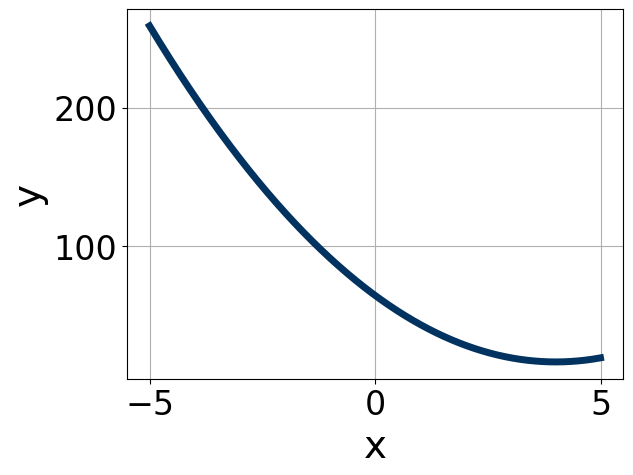
\includegraphics[width = 0.3\textwidth]{../Figures/quadraticEquationToGraphCopyAB.png}\item 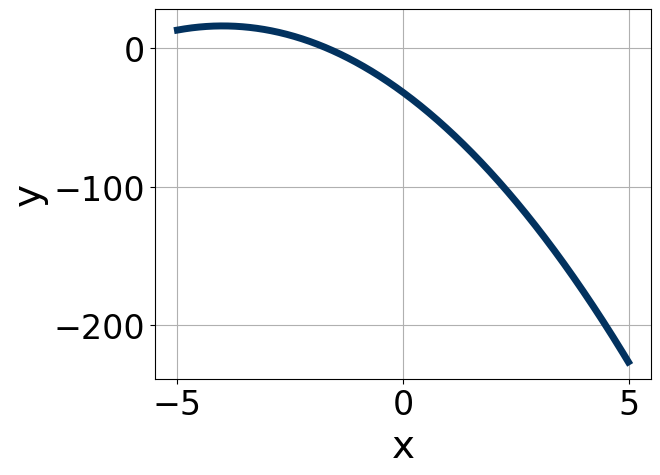
\includegraphics[width = 0.3\textwidth]{../Figures/quadraticEquationToGraphCopyBB.png}\item 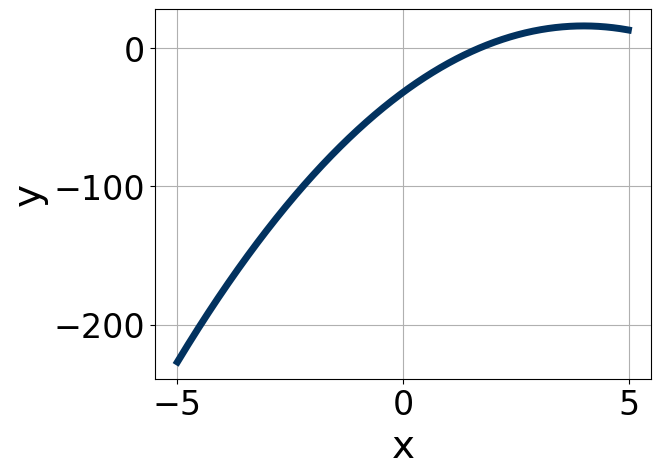
\includegraphics[width = 0.3\textwidth]{../Figures/quadraticEquationToGraphCopyCB.png}\item 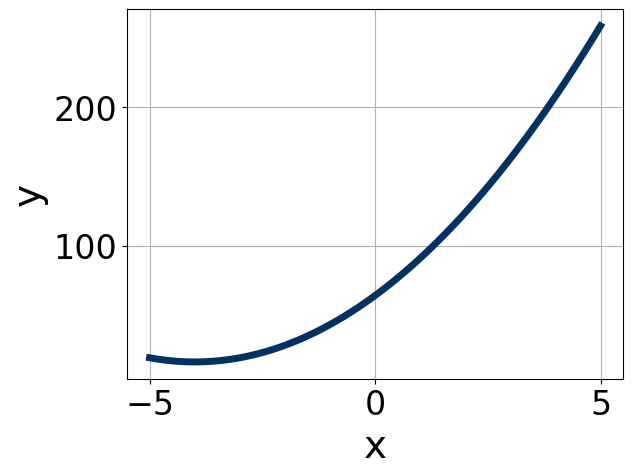
\includegraphics[width = 0.3\textwidth]{../Figures/quadraticEquationToGraphCopyDB.png}\end{multicols}\item None of the above.
\end{enumerate} }
\litem{
Solve the quadratic equation below. Then, choose the intervals that the solutions belong to, with $x_1 \leq x_2$ (if they exist).\[ -11x^{2} +11 x + 8 = 0 \]\begin{enumerate}[label=\Alph*.]
\item \( x_1 \in [-0.49, 0.51] \text{ and } x_2 \in [0.84, 1.56] \)
\item \( x_1 \in [-24.25, -20.25] \text{ and } x_2 \in [22.04, 23.11] \)
\item \( x_1 \in [-18.37, -14.37] \text{ and } x_2 \in [4.87, 5.5] \)
\item \( x_1 \in [-5.49, -0.49] \text{ and } x_2 \in [0.36, 1.22] \)
\item \( \text{There are no Real solutions.} \)

\end{enumerate} }
\litem{
Solve the quadratic equation below. Then, choose the intervals that the solutions $x_1$ and $x_2$ belong to, with $x_1 \leq x_2$.\[ 25x^{2} -60 x + 36 = 0 \]\begin{enumerate}[label=\Alph*.]
\item \( x_1 \in [0.12, 0.39] \text{ and } x_2 \in [5.23, 7.41] \)
\item \( x_1 \in [0.51, 0.71] \text{ and } x_2 \in [1.48, 2.88] \)
\item \( x_1 \in [0.38, 0.53] \text{ and } x_2 \in [2.79, 5.33] \)
\item \( x_1 \in [1.08, 1.33] \text{ and } x_2 \in [0.17, 2.27] \)
\item \( x_1 \in [29.88, 30.1] \text{ and } x_2 \in [28.99, 30.05] \)

\end{enumerate} }
\litem{
Solve the quadratic equation below. Then, choose the intervals that the solutions $x_1$ and $x_2$ belong to, with $x_1 \leq x_2$.\[ 15x^{2} -2 x -24 = 0 \]\begin{enumerate}[label=\Alph*.]
\item \( x_1 \in [-6.73, -5.44] \text{ and } x_2 \in [0.25, 0.33] \)
\item \( x_1 \in [-3.72, -3.18] \text{ and } x_2 \in [0.28, 0.61] \)
\item \( x_1 \in [-18.11, -17.49] \text{ and } x_2 \in [20, 20.03] \)
\item \( x_1 \in [-1.14, -0.44] \text{ and } x_2 \in [2.49, 2.72] \)
\item \( x_1 \in [-1.22, -0.84] \text{ and } x_2 \in [1.32, 1.48] \)

\end{enumerate} }
\litem{
Graph the equation below.\[ f(x) = (x-3)^2 + 12 \]\begin{enumerate}[label=\Alph*.]
\begin{multicols}{2}\item 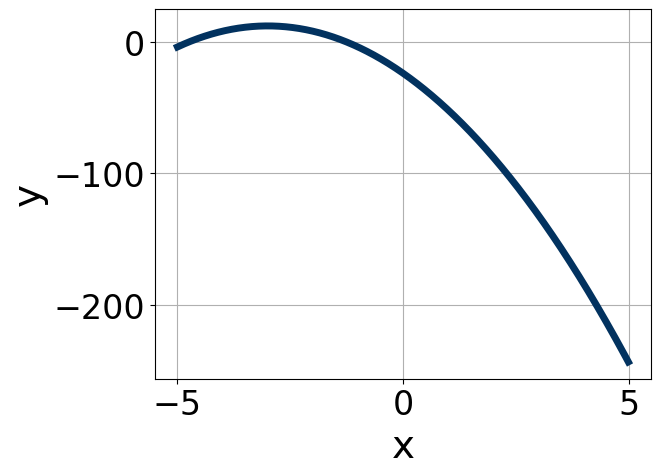
\includegraphics[width = 0.3\textwidth]{../Figures/quadraticEquationToGraphAB.png}\item 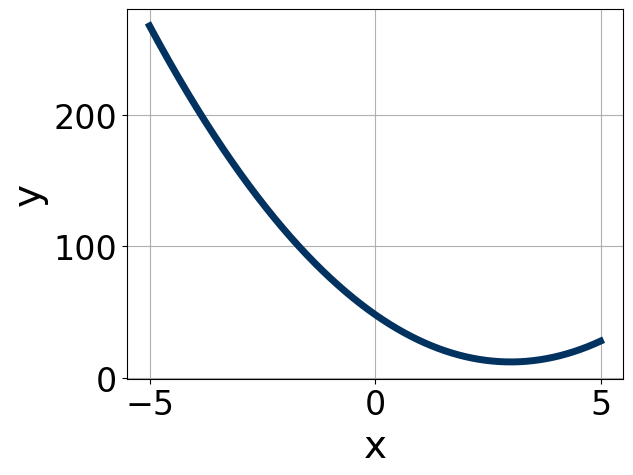
\includegraphics[width = 0.3\textwidth]{../Figures/quadraticEquationToGraphBB.png}\item 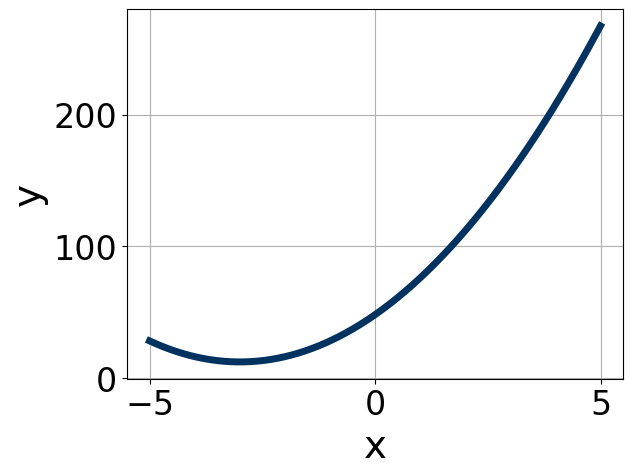
\includegraphics[width = 0.3\textwidth]{../Figures/quadraticEquationToGraphCB.png}\item 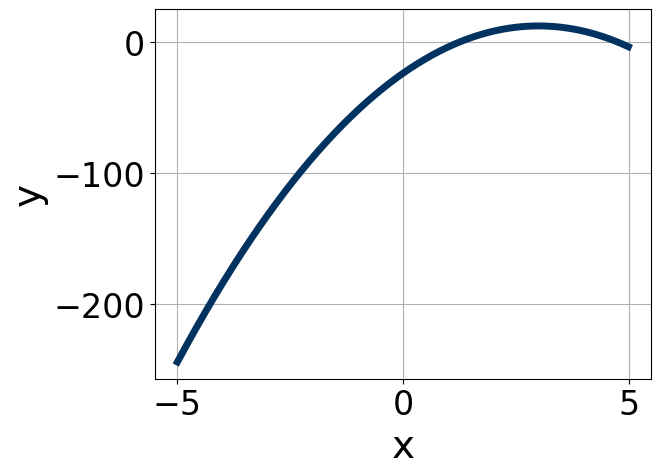
\includegraphics[width = 0.3\textwidth]{../Figures/quadraticEquationToGraphDB.png}\end{multicols}\item None of the above.
\end{enumerate} }
\litem{
Factor the quadratic below. Then, choose the intervals that contain the constants in the form $(ax+b)(cx+d); b \leq d.$\[ 24x^{2} -2 x -15 \]\begin{enumerate}[label=\Alph*.]
\item \( a \in [1.7, 5.4], \hspace*{5mm} b \in [-6, 1], \hspace*{5mm} c \in [8, 10], \text{ and } \hspace*{5mm} d \in [2, 4] \)
\item \( a \in [3.3, 7.2], \hspace*{5mm} b \in [-6, 1], \hspace*{5mm} c \in [3, 6], \text{ and } \hspace*{5mm} d \in [2, 4] \)
\item \( a \in [-1.1, 1.9], \hspace*{5mm} b \in [-23, -17], \hspace*{5mm} c \in [-4, 2], \text{ and } \hspace*{5mm} d \in [15, 25] \)
\item \( a \in [17.6, 18.6], \hspace*{5mm} b \in [-6, 1], \hspace*{5mm} c \in [-4, 2], \text{ and } \hspace*{5mm} d \in [2, 4] \)
\item \( \text{None of the above.} \)

\end{enumerate} }
\litem{
Write the equation of the graph presented below in the form $f(x)=ax^2+bx+c$, assuming  $a=1$ or $a=-1$. Then, choose the intervals that $a, b,$ and $c$ belong to.
\begin{center}
    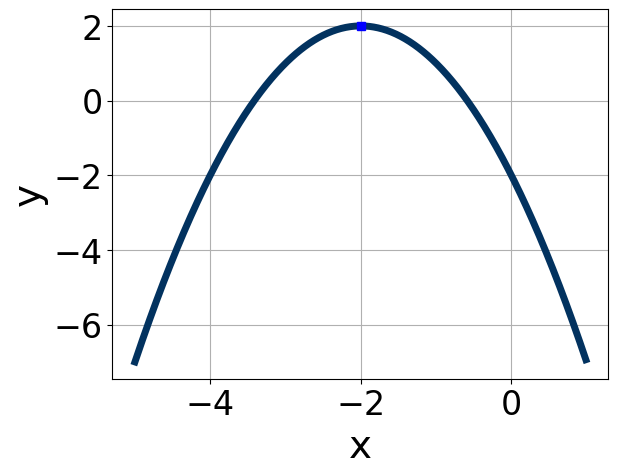
\includegraphics[width=0.5\textwidth]{../Figures/quadraticGraphToEquationC.png}
\end{center}
\begin{enumerate}[label=\Alph*.]
\item \( a \in [-1.1, -0.7], \hspace*{5mm} b \in [2, 5], \text{ and } \hspace*{5mm} c \in [-9, -3] \)
\item \( a \in [-1.1, -0.7], \hspace*{5mm} b \in [-7, -1], \text{ and } \hspace*{5mm} c \in [-4, -1] \)
\item \( a \in [-1.1, -0.7], \hspace*{5mm} b \in [2, 5], \text{ and } \hspace*{5mm} c \in [-4, -1] \)
\item \( a \in [0.2, 2.4], \hspace*{5mm} b \in [2, 5], \text{ and } \hspace*{5mm} c \in [6, 9] \)
\item \( a \in [0.2, 2.4], \hspace*{5mm} b \in [-7, -1], \text{ and } \hspace*{5mm} c \in [6, 9] \)

\end{enumerate} }
\litem{
Factor the quadratic below. Then, choose the intervals that contain the constants in the form $(ax+b)(cx+d); b \leq d.$\[ 24x^{2} +50 x + 25 \]\begin{enumerate}[label=\Alph*.]
\item \( a \in [5.98, 6.49], \hspace*{5mm} b \in [4, 10], \hspace*{5mm} c \in [3.95, 4.54], \text{ and } \hspace*{5mm} d \in [2, 9] \)
\item \( a \in [11.66, 13.4], \hspace*{5mm} b \in [4, 10], \hspace*{5mm} c \in [1.8, 2.43], \text{ and } \hspace*{5mm} d \in [2, 9] \)
\item \( a \in [-0.36, 1.49], \hspace*{5mm} b \in [13, 21], \hspace*{5mm} c \in [0.97, 1.26], \text{ and } \hspace*{5mm} d \in [23, 33] \)
\item \( a \in [1.25, 2.55], \hspace*{5mm} b \in [4, 10], \hspace*{5mm} c \in [11.85, 12.45], \text{ and } \hspace*{5mm} d \in [2, 9] \)
\item \( \text{None of the above.} \)

\end{enumerate} }
\litem{
Write the equation of the graph presented below in the form $f(x)=ax^2+bx+c$, assuming  $a=1$ or $a=-1$. Then, choose the intervals that $a, b,$ and $c$ belong to.
\begin{center}
    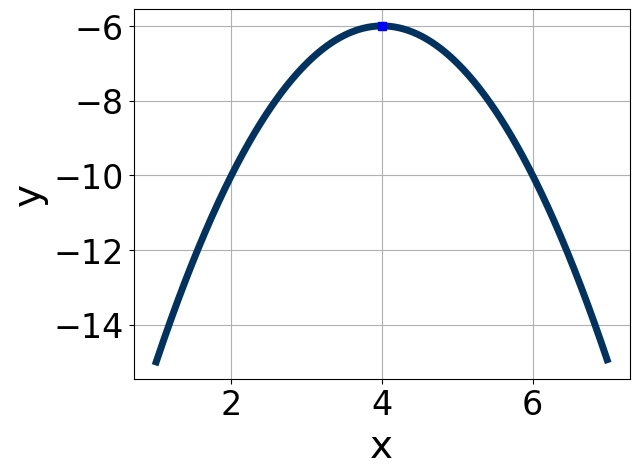
\includegraphics[width=0.5\textwidth]{../Figures/quadraticGraphToEquationCopyC.png}
\end{center}
\begin{enumerate}[label=\Alph*.]
\item \( a \in [-1.3, 0.5], \hspace*{5mm} b \in [8, 9], \text{ and } \hspace*{5mm} c \in [-23, -18] \)
\item \( a \in [0, 1.1], \hspace*{5mm} b \in [8, 9], \text{ and } \hspace*{5mm} c \in [8, 11] \)
\item \( a \in [0, 1.1], \hspace*{5mm} b \in [-8, -5], \text{ and } \hspace*{5mm} c \in [8, 11] \)
\item \( a \in [-1.3, 0.5], \hspace*{5mm} b \in [-8, -5], \text{ and } \hspace*{5mm} c \in [-23, -18] \)
\item \( a \in [-1.3, 0.5], \hspace*{5mm} b \in [-8, -5], \text{ and } \hspace*{5mm} c \in [-12, -7] \)

\end{enumerate} }
\litem{
Solve the quadratic equation below. Then, choose the intervals that the solutions belong to, with $x_1 \leq x_2$ (if they exist).\[ -12x^{2} -10 x + 4 = 0 \]\begin{enumerate}[label=\Alph*.]
\item \( x_1 \in [-1.54, -0.67] \text{ and } x_2 \in [-0.7, 1] \)
\item \( x_1 \in [-0.59, -0.03] \text{ and } x_2 \in [0.8, 1.9] \)
\item \( x_1 \in [-18.17, -17.3] \text{ and } x_2 \in [16.4, 18.4] \)
\item \( x_1 \in [-4.18, -2.99] \text{ and } x_2 \in [12.8, 13.7] \)
\item \( \text{There are no Real solutions.} \)

\end{enumerate} }
\litem{
Graph the equation below.\[ f(x) = (x-3)^2 + 18 \]\begin{enumerate}[label=\Alph*.]
\begin{multicols}{2}\item 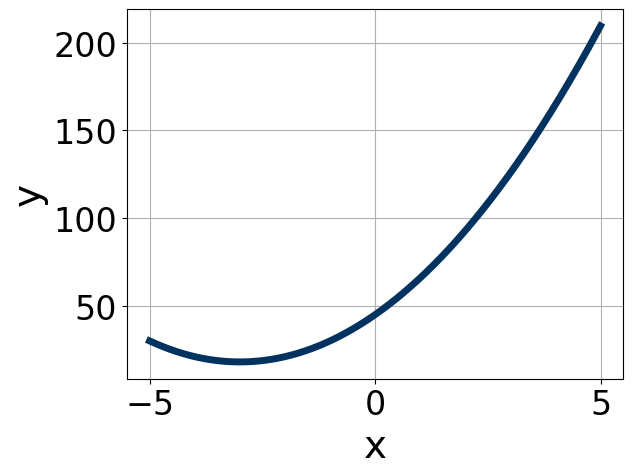
\includegraphics[width = 0.3\textwidth]{../Figures/quadraticEquationToGraphCopyAC.png}\item 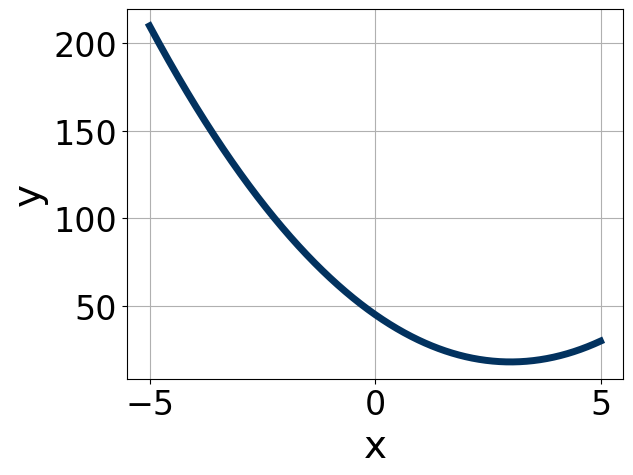
\includegraphics[width = 0.3\textwidth]{../Figures/quadraticEquationToGraphCopyBC.png}\item 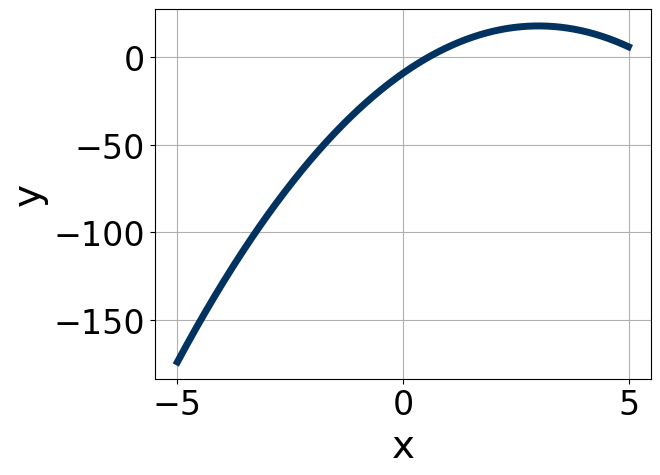
\includegraphics[width = 0.3\textwidth]{../Figures/quadraticEquationToGraphCopyCC.png}\item 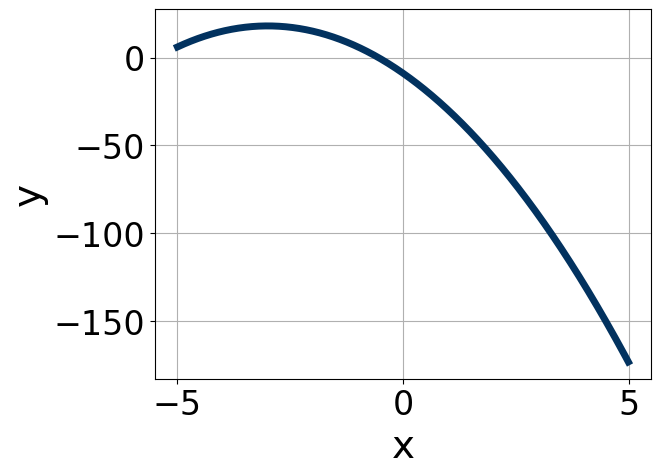
\includegraphics[width = 0.3\textwidth]{../Figures/quadraticEquationToGraphCopyDC.png}\end{multicols}\item None of the above.
\end{enumerate} }
\litem{
Solve the quadratic equation below. Then, choose the intervals that the solutions belong to, with $x_1 \leq x_2$ (if they exist).\[ -11x^{2} +7 x + 9 = 0 \]\begin{enumerate}[label=\Alph*.]
\item \( x_1 \in [-21.6, -20.4] \text{ and } x_2 \in [21.05, 22.11] \)
\item \( x_1 \in [-1.1, 1.9] \text{ and } x_2 \in [0.88, 2.39] \)
\item \( x_1 \in [-3.2, -0.8] \text{ and } x_2 \in [0.09, 0.99] \)
\item \( x_1 \in [-15.2, -12.3] \text{ and } x_2 \in [6.89, 7.07] \)
\item \( \text{There are no Real solutions.} \)

\end{enumerate} }
\litem{
Solve the quadratic equation below. Then, choose the intervals that the solutions $x_1$ and $x_2$ belong to, with $x_1 \leq x_2$.\[ 25x^{2} -75 x + 54 = 0 \]\begin{enumerate}[label=\Alph*.]
\item \( x_1 \in [0.31, 0.39] \text{ and } x_2 \in [5.96, 7.79] \)
\item \( x_1 \in [29.95, 30] \text{ and } x_2 \in [42.83, 46.12] \)
\item \( x_1 \in [0.57, 0.64] \text{ and } x_2 \in [3.3, 3.81] \)
\item \( x_1 \in [1.16, 1.25] \text{ and } x_2 \in [0.89, 2.51] \)
\item \( x_1 \in [0.4, 0.46] \text{ and } x_2 \in [4.94, 5.77] \)

\end{enumerate} }
\litem{
Solve the quadratic equation below. Then, choose the intervals that the solutions $x_1$ and $x_2$ belong to, with $x_1 \leq x_2$.\[ 25x^{2} +60 x + 36 = 0 \]\begin{enumerate}[label=\Alph*.]
\item \( x_1 \in [-3.83, -3.59] \text{ and } x_2 \in [-0.46, -0.32] \)
\item \( x_1 \in [-6.78, -5.74] \text{ and } x_2 \in [-0.37, -0.09] \)
\item \( x_1 \in [-30.58, -29.25] \text{ and } x_2 \in [-30.05, -29.91] \)
\item \( x_1 \in [-1.75, -0.99] \text{ and } x_2 \in [-1.23, -1.11] \)
\item \( x_1 \in [-2.56, -2.16] \text{ and } x_2 \in [-0.79, -0.53] \)

\end{enumerate} }
\litem{
Graph the equation below.\[ f(x) = -(x-3)^2 + 17 \]\begin{enumerate}[label=\Alph*.]
\begin{multicols}{2}\item 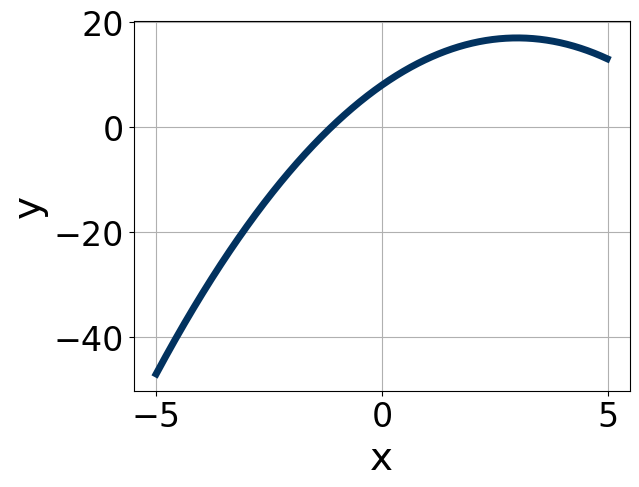
\includegraphics[width = 0.3\textwidth]{../Figures/quadraticEquationToGraphAC.png}\item 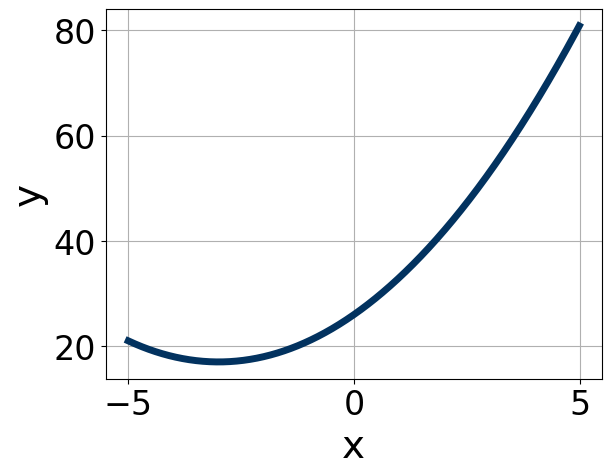
\includegraphics[width = 0.3\textwidth]{../Figures/quadraticEquationToGraphBC.png}\item 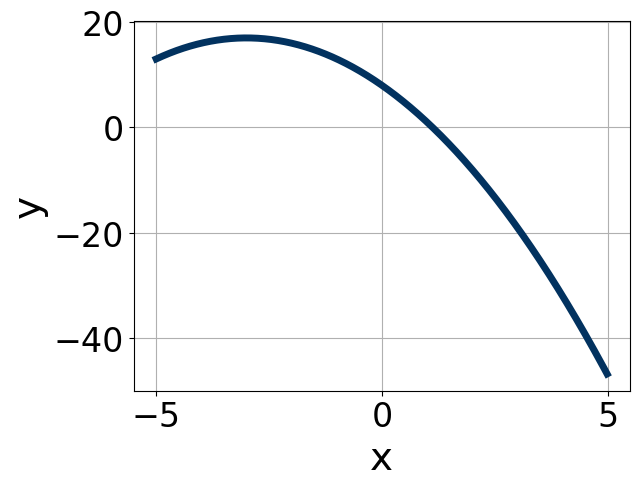
\includegraphics[width = 0.3\textwidth]{../Figures/quadraticEquationToGraphCC.png}\item 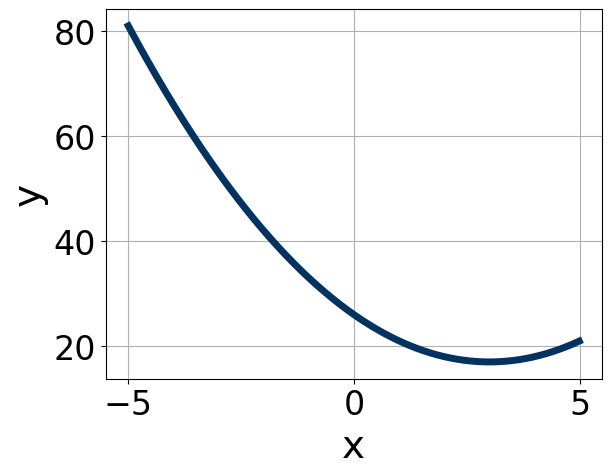
\includegraphics[width = 0.3\textwidth]{../Figures/quadraticEquationToGraphDC.png}\end{multicols}\item None of the above.
\end{enumerate} }
\end{enumerate}

\end{document}